\documentclass[runningheads]{llncs}
\usepackage[paperheight=295mm,paperwidth=210mm]{geometry}
\usepackage{graphicx}
\usepackage{import}
\usepackage{kotex}
\usepackage{amsmath}
\usepackage{amssymb}
\usepackage[dvipsnames]{xcolor}
\usepackage{fancyvrb}
\usepackage{listings}
\usepackage{indentfirst}
\usepackage{tabularx}
\usepackage{underscore}
\usepackage{multicol}
\usepackage{tikz}
\usepackage[square,sort,comma,super]{natbib}
\usepackage{inconsolata} % Inconsolata
\usepackage{mathptmx} % Times New Roman
\usepackage[cache=false]{minted}
\graphicspath{ {./images/} }
\lstset{basicstyle=\footnotesize\ttfamily,breaklines=true}
\renewcommand{\bibname}{참고문헌}
\setlength{\parindent}{1em}
\setlength{\parskip}{1em}
\linespread{1.2}
{\renewcommand{\arraystretch}{1.5}%
\setlength{\tabcolsep}{0.5em}%
\newenvironment{Figure}
  {\par\medskip\noindent\minipage{\linewidth}}
  {\endminipage\par\medskip}
 
	
\begin{document}

\title{MAT2410 (응용수학I) \space \newline 중간시험 솔루션}
\author{서강대학교 컴퓨터공학과 박수현 (20181634)}
\institute{서강대학교 컴퓨터공학과}
\maketitle

% Problem 1
\subsubsection{1. (12점)} 확률변수(random variable) $X$의 분포함수(CDF)가 다음과 같을 때, $P\left(\dfrac{1}{2} \leq X < 1\right)$과 $f\left(x\right)$을 구하시오.
\[F\left(x\right) = \left\{
\begin{array}{ll}
	0 				& \qquad x < 0 \\
	0.25x + 0.25 	& \qquad 0 \leq x < 0.5 \\
	0.5 			& \qquad 0.5 \leq x < 1 \\
	0.5x^2			& \qquad 1 \leq x < \sqrt{2} \\
	1 				& \qquad x \geq \sqrt{2}
\end{array}
\right. \]

\paragraph{Solution.} 위의 함수의 그래프는 다음과 같이 주어진다.
\begin{center}
	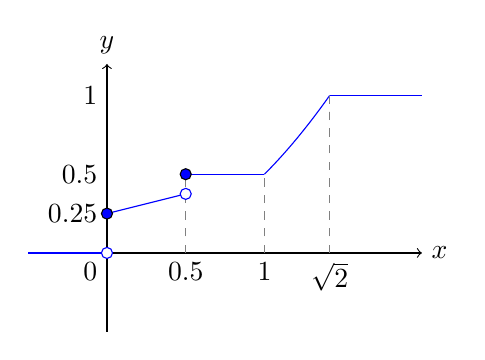
\begin{tikzpicture}
		\draw[->] (-0.5,0) -- (4,0) node[right] {$x$};
		\draw[->] (0,-1) -- (0,2.4) node[above] {$y$};
		
		\node[below left] at (0,0) {0};
		\node[below] at (1,0) {0.5};
		\node[below] at (2,0) {1};
		\node[below] at (2.828,0) {$\sqrt{2}$};
		\node[left] at (0,0.5) {0.25};
		\node[left] at (0,1) {0.5};
		\node[left] at (0,2) {1};
		
		\draw[scale=2,domain=-0.5:0,smooth,variable=\x,blue] plot ({\x},{0});
		\draw[scale=2,domain=0:0.5,smooth,variable=\x,blue] plot ({\x},{0.25*\x+0.25});
		\draw[scale=2,domain=0.5:1,smooth,variable=\x,blue] plot ({\x},{0.5});
		\draw[scale=2,domain=1:1.414,smooth,variable=\x,blue] plot ({\x},{0.5*\x^2});
		\draw[scale=2,domain=1.414:2,smooth,variable=\x,blue] plot ({\x},{1});

		\draw[scale=2,domain=0:0.5,smooth,dashed,variable=\y,gray] plot ({0.5},{\y});
		\draw[scale=2,domain=0:0.5,smooth,dashed,variable=\y,gray] plot ({1},{\y});
		\draw[scale=2,domain=0:1,smooth,dashed,variable=\y,gray] plot ({1.414},{\y});

		\draw[scale=2,blue,fill=white] (0,0) circle[radius=1pt];
		\draw[scale=2,blue,fill=white] (0.5,0.375) circle[radius=1pt];
		\draw[scale=2,fill=blue] (0,0.25) circle[radius=1pt];
		\draw[scale=2,fill=blue] (0.5,0.5) circle[radius=1pt];
	\end{tikzpicture}
\end{center}

이 때
\begin{align*}
	& P\left(\dfrac{1}{2} \leq X < 1\right)\\
	=& P\left(X < 1\right) - P\left(X < \dfrac{1}{2}\right) \\
	=& F\left(1^-\right) - F\left(\dfrac{1}{2}^-\right)\\
	=& 0.5-0.375 = 0.125
\end{align*}
이다.

그래프에서, $F$는 $x = 0$, $x = 0.5$에서 불연속임을 확인할 수 있다. 그러므로
\begin{align*}
	f\left(0\right) &= F\left(0^+\right) - F\left(0^-\right) = 0.25 \\
	f\left(0.5\right) &= F\left(0.5^+\right) - F\left(0.5^-\right) = 0.125
\end{align*}
이고, 나머지 구간에서 $f$는 $F$를 $x$에 대해 미분해 얻을 수 있다. 따라서
\[f\left(x\right) = \left\{
\begin{array}{ll}
	0 				& \qquad x < 0 \\
	0.25		 	& \qquad 0 \leq x < 0.5 \\
	0.125		 	& \qquad x = 0.5 \\
	0 				& \qquad 0.5 < x < 1 \\
	x				& \qquad 1 < x < \sqrt{2} \\
	0 				& \qquad x > \sqrt{2}
\end{array}
\right. \]
를 얻을 수 있다.

% Problem 2
\subsubsection{2. (6점)} 명품을 취급하는 가게에는 60\%가 진품인 것으로 알려져 있다. 이 가게의 진품 감별사는 진품을 모조품으로 감별할 확률이 0.05이고 모조품을 진품이라고 감별할
확률은 0.1이라고 한다. 이 감별사가 모조품이라고 감별한 제품이 실제로는 진품이었을 확률은 얼마인가?

\paragraph{Solution.} 문제에서 주어진 사건들을 다음과 같이 정의하자.
\begin{align*}
	\textrm{사건 }A &= \textrm{명품이 진품인 사건} \\
	\textrm{사건 }B &= \textrm{명품을 진품으로 감별한 사건}
\end{align*}
그러면 문제에서 등장한 명제들을 다음과 같이 표현할 수 있다.
\[P\left(A\right) = 0.6 \qquad P\left(B^c|A\right) = 0.05 \qquad P\left(B|A^c\right) = 0.1\]
우리가 구하고자 하는 값은 $P\left(A|B^c\right)$이다.

\begin{align}
	& P\left(A|B^c\right) \nonumber \\
	=& \frac{P\left(A \cap B^c\right)}{P\left(B^c\right)} \nonumber \\
	=& \frac{P\left(A \cap B^c\right)}{P\left(A\right)} \times \frac{P\left(A\right)}{P\left(B^c\right)} \nonumber \\
	=& P\left(B^c|A\right) \times \frac{P\left(A\right)}{P\left(B^c\right)} \nonumber \\
	=& \frac{0.05 \times 0.6}{P\left(B^c\right)} \label{eq2:1}
\end{align}

또한 $P\left(B^c|A\right) = 0.05$에서 $P\left(A \cap B^c\right) = 0.05P\left(A\right) = 0.03$을,
$P\left(B|A^c\right) = 0.1$에서 $P\left(A^c \cap B\right) = 0.1P\left(A^c\right) = 0.1\left[1 - P\left(A\right)\right] = 0.04$를 얻을 수 있다.
따라서

\begin{align}
	&P\left(A\right) = P\left(A \cap B\right) + P\left(A \cap B^c\right) \nonumber \\
	\Rightarrow& 0.6 = P\left(A \cap B\right) + 0.03 \nonumber \\
	\Rightarrow& P\left(A \cap B\right) = 0.57 \label{eq2:2}
\end{align}

이고, 또한

\begin{align}
	&P\left(B\right) = P\left(A \cap B\right) + P\left(A^c \cap B\right) \nonumber \\
	\Rightarrow& P\left(B\right) = 0.57 + 0.04 \qquad \because \eqref{eq2:2} \nonumber \\
	\Rightarrow& P\left(B\right) = 0.61 \label{eq2:3}
\end{align}

이므로 \eqref{eq2:1}과 \eqref{eq2:3}에 의해

\begin{align*}
	P\left(A|B^c\right) =& \frac{0.05 \times 0.6}{P\left(B^c\right)} \\
	=& \frac{0.05 \times 0.6}{1 - P\left(B\right)} \\
	=& \frac{0.05 \times 0.6}{1 - 0.61} = \frac{0.03}{0.39} = \frac{1}{13}
\end{align*}

이다.

% Problem 3
\subsubsection{3. (12점)} 두 확률변수 $X$와 $Y$의 결합확률밀도함수(joint PDF)가 다음과 같을 때,
\[f\left(x, y\right) = 2x \qquad 0<x<1,\, 0<y<1\]
$P\left(X^2+Y^2<\dfrac{1}{2}\right)$와 $P\left(X+Y<\dfrac{3}{2}\right)$을 각각 구하시오.

\paragraph{Solution.}
\begin{itemize}
    \item [(1)]{
    \begin{align*}
		& P\left(X^2+Y^2<\dfrac{1}{2}\right) \\
		=& \int_{0}^{\frac{1}{\sqrt{2}}} \int_{0}^{\sqrt{\frac{1}{2}-x^2}} f\left(x, y\right) \mathop{dy} \mathop{dx} \\
		=& \int_0^{\frac{\pi}{2}} \int_0^{\frac{1}{\sqrt{2}}} rf\left(x, y\right) \mathop{dr} \mathop{d\theta} \qquad r^2 = x^2 + y^2,\, \tan\theta = \frac{y}{x} \\
		=& \int_0^{\frac{\pi}{2}} \int_0^{\frac{1}{\sqrt{2}}} 2rx \mathop{dr} \mathop{d\theta} \\
		=& 2 \int_0^{\frac{\pi}{2}} \int_0^{\frac{1}{\sqrt{2}}} r^2 \cos\theta \mathop{dr} \mathop{d\theta} \\
		=& 2 \int_0^{\frac{\pi}{2}} \cos\theta \mathop{d\theta} \int_0^{\frac{1}{\sqrt{2}}} r^2 \mathop{dr} \\
		=& 2 \left[\sin \theta\right]_0^{\frac{\pi}{2}} \left[\frac{1}{3} r^3\right]_0^{\frac{1}{\sqrt{2}}} \\
		=& \frac{2}{3} \times \frac{1}{2\sqrt{2}} = \frac{1}{3\sqrt{2}}
	\end{align*}
    }
    \item [(2)]{
	$P\left(X+Y<\dfrac{3}{2}\right)$에 해당하는 영역을 그래프로 나타내면 다음과 같다.
	\begin{center}
		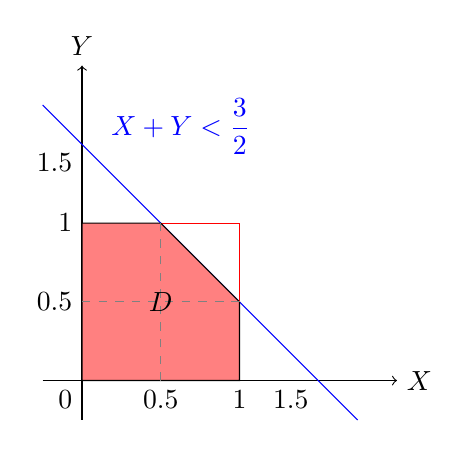
\begin{tikzpicture}
			\draw[->] (-0.5,0) -- (4,0) node[right] {$X$};
			\draw[->] (0,-0.5) -- (0,4) node[above] {$Y$};
			
			\node[below left] at (0,0) {0};
			\node[below] at (1,0) {0.5};
			\node[below] at (2,0) {1};
			\node[below left] at (3,0) {1.5};
			\node[left] at (0,1) {0.5};
			\node[left] at (0,2) {1};
			\node[below left] at (0,3) {1.5};
			\node[above right,text=blue] at (0.25,2.75) {$X+Y<\dfrac{3}{2}$};
			
			\draw[scale=2,domain=-0.25:1.75,smooth,variable=\x,blue] plot ({\x},{1.5-\x});
			\draw[scale=2,domain=0:1,smooth,variable=\x,red] plot ({\x},{1});
			\draw[scale=2,domain=0:1,smooth,variable=\y,red] plot ({1},{\y});

			\draw[scale=2,fill=red!50] (0,0) -- (1,0) -- (1,0.5) -- (0.5,1) -- (0,1) -- cycle;

			\draw[scale=2,domain=0:1,smooth,dashed,variable=\y,gray] plot ({0.5},{\y});
			\draw[scale=2,domain=0:1,smooth,dashed,variable=\x,gray] plot ({\x},{0.5});

			\node at (1,1) {$D$};
		\end{tikzpicture}
	\end{center}
	따라서
	\begin{align*}
		& P\left(X+Y<\dfrac{3}{2}\right) \\
		=& \iint_D f\left(x, y\right) \mathop{dy} \mathop{dx} \\
		=& \int_0^1 \int_0^{\mathop{\mathrm{min}} \left(1,\, \frac{3}{2} - x\right)} f\left(x, y\right) \mathop{dy} \mathop{dx} \\
		=& \int_0^\frac{1}{2} \int_0^1 2x \mathop{dy} \mathop{dx} + \int_\frac{1}{2}^1 \int_0^{\frac{3}{2} - x} 2x \mathop{dy} \mathop{dx} \\
		=& \int_0^\frac{1}{2} 2x \mathop{dx} + \int_\frac{1}{2}^1 2x\left(\frac{3}{2} - x\right) \mathop{dy} \mathop{dx} \\
		=& \left.x^2\right|_0^\frac{1}{2} + \left[\frac{3}{2}x^2 - \frac{2}{3}x^3\right]_\frac{1}{2}^1 \\
		=& \frac{1}{4} + \left(\frac{3}{2} - \frac{2}{3}\right) - \left(\frac{3}{8} - \frac{1}{12}\right) = \frac{19}{24}
	\end{align*}
    }
\end{itemize}

% Problem 4
\subsubsection{4. (15점)} 도심의 순찰차는 호출이 있을 때마다 순찰을 하는데 그 순찰 횟수는 시간당 평균 5회인 포아송(Poisson) 분포를 따른다고 할 때

\begin{itemize}
    \item [(1)] 2시간 동안 한 번의 호출도 없을 확률을 구하시오.
    \item [(2)] 순찰차가 호출을 3번 받을 때까지의 시간을 나타내는 확률변수를 $T$라고 할 때, $T$의 분포를 구하시오.
    \item [(3)] 호출이 없었던 상태로 3시간이 지난 상태에서 다음 호출까지의 총 시간이 8시간을 넘길 확률을 구하시오.
\end{itemize}

\paragraph{Solution.} \begin{itemize}
    \item [(1)] {
		2시간 동안 일어나는 호출의 기댓값은 10회이다. 따라서 $\lambda = 10$인 포아송 분포 $\mathrm{Poi}\left(10\right)$에 대해
		\[f\left(0\right) = \frac{10^0 e^{-10}}{0!} = e^{-10}\]
		이다.
	}
    \item [(2)] {
		$T \sim \mathrm{\Gamma}\left(3,\, \dfrac{1}{5}\right)$이다.
	}
	\item [(3)] 포아송 분포는 무기억성을 가지므로 호출이 없었던 상태로 3시간이 지난 상태에서 다음 호출까지의 총 시간이 8시간을 넘길 확률은
	5시간 동안 한 번의 호출도 없었을 확률과 같다. 따라서 이 때의 확률을 (1)과 같은 방법으로 계산하면 $e^{-25}$이다.
\end{itemize}

% Problem 5
\subsubsection{5. (15점)} 이산인 두 확률변수 $X$와 $Y$의 결합확률질량함수(joint PMF)가 다음과 같을 때, 
\[f_{X,\,Y}\left(x,\,y\right) = \frac{2}{n\left(n + 1\right)} \qquad x=1,\,2,\,\cdots,\,n \qquad y=1,\,2,\,\cdots,\,x \]
\begin{itemize}
    \item [(1)] 두 확률변수 $X$와 $Y$의 표본공간(sample space)를 구하고 결합확률질량함수(joint PMF)임을 확인하시오.
    \item [(2)] 각각의 확률변수에 대한 주변확률질량함수(marginal PMF)를 구하고 이를 이용하여 $X$와 $Y$의 독립성 여부를 결정하시오.
\end{itemize}

\paragraph{Solution.} 
\begin{itemize}
	\item [(1)] {
		$x=1,\,2,\,\cdots,\,n$이고 $y=1,\,2,\,\cdots,\,x$이므로 표본공간 $\mathrm{\Omega}$는 다음과 같이 나타낼 수 있다.
		\[\mathrm{\Omega} = \left\{\left(x,\, y\right) \middle| 1 \leq x \leq n ,\, 1 \leq y \leq x,\, \left(x,\, y\right) \in \mathbb{Z}^2 \right\}\]
		$f$가 확률질량함수라면 $\mathrm{\Omega}$의 모든 원소 $\left(x,\, y\right)$에 대해 $\sum_{\left(x,\, y\right) \in \mathrm{\Omega}} f\left(x,\, y\right) = 1$이어야 한다.
		\begin{align*}
			& \sum_{\left(x,\, y\right) \in \mathrm{\Omega}} f\left(x,\, y\right) \\
			=& \sum_{x=1}^{n} \sum_{y=1}^{x} f\left(x,\, y\right) \\
			=& \sum_{x=1}^{n} \sum_{y=1}^{x} \frac{2}{n\left(n + 1\right)} \\
			=& \sum_{x=1}^{n} \frac{2x}{n\left(n + 1\right)} \\
			=& \frac{2}{n\left(n + 1\right)} \times \frac{n\left(n + 1\right)}{2} = 1 \\
		\end{align*}
		따라서 $f$는 확률질량함수이다.
	}
    \item [(2)] {
		\begin{align*}
			f_X\left(y\right) =& \sum_{y=1}^{x} f\left(x,\, y\right) \\
			=& \sum_{y=1}^{x} \frac{2}{n\left(n + 1\right)} \\
			=& \frac{2x}{n\left(n + 1\right)} \qquad 1 \leq x \leq n,\, x \in \mathbb{Z}\\
		\end{align*}
		\begin{align*}
			f_Y\left(y\right) =& \sum_{x=y}^{n} f\left(x,\, y\right) \\
			=& \sum_{x=y}^{n} \frac{2}{n\left(n + 1\right)} \\
			=& \frac{2\left(n - y + 1\right)}{n\left(n + 1\right)} \qquad 1 \leq y \leq n,\, y \in \mathbb{Z}\\
		\end{align*}
		$X$와 $Y$가 독립일 경우 $f_{X,\,Y} = f_X f_Y$이어야 한다. 그러나 $f_{X,\,Y} \neq f_X f_Y$이므로 $X$와 $Y$는 독립이 아니다.
	}
\end{itemize}

% Problem 6
\subsubsection{6. (10점)} 두 확률변수 $X$와 $Y$의 결합확률밀도함수(joint PDF)가
\[f_{X,\,Y}\left(x,\,y\right) = \frac{e^{-\frac{x}{y} - y}}{y} \qquad x > 0,\,y > 0\]
일 때, 조건부 확률밀도함수(conditional PDF) $f\left(x\middle|y\right)$을 구하고 이를 이용하여 $P\left(X>1\middle|Y=y\right)$를 구하시오.

\paragraph{Solution.}
\begin{itemize}
	\item [(1)] {
		\begin{align*}
			& f\left(x\middle|y\right) \\
			=& \frac{f\left(x,\,y\right)}{f_Y\left(y\right)} \\
			=& \frac{f\left(x,\,y\right)}{\displaystyle \int_0^\infty f\left(x,\,y\right) \mathop{dx}} \\
			=& \frac{f\left(x,\,y\right)}{\displaystyle \int_0^\infty \frac{e^{-\frac{x}{y} - y}}{y} \mathop{dx}}
			= \frac{f\left(x,\,y\right)}{\displaystyle \frac{e^{-y}}{y}\int_0^\infty e^{-\frac{x}{y}} \mathop{dx}} \\
			=& \frac{f\left(x,\,y\right)}{\displaystyle \frac{e^{-y}}{y} \left[-ye^{-\frac{x}{y}}\right]_{x=0}^{x=\infty}} \\
			=& \frac{f\left(x,\,y\right)}{\displaystyle \frac{e^{-y}}{y} \left(0 + ye^0\right)}
			= \frac{\frac{e^{-\frac{x}{y} - y}}{y}}{e^{-y}} = \frac{e^{-\frac{x}{y}}}{y}\\
		\end{align*}
	}
    \item [(2)] {
		\begin{align*}
			& P\left(X>1\middle|Y=y\right) \\
			&= \int_1^\infty f\left(x\middle|y\right) \mathop{dx} \\
			&= \int_1^\infty \frac{e^{-\frac{x}{y}}}{y} \mathop{dx}
			= \frac{1}{y} \int_1^\infty e^{-\frac{x}{y}} \mathop{dx} \\
			&= \left.-e^{-\frac{x}{y}}\right|_{x=1}^{x=\infty} \\
			&= 0 + e^{-\frac{1}{y}} = e^{-\frac{1}{y}}
		\end{align*}
	}
\end{itemize} 

% Problem 7-1
\subsubsection{7-1. (10점)} 연속확률변수 $X_1,\,X_2,\,\cdots,\,X_n$에 대하여
\begin{itemize}
	\item [(1)] $\mathrm{E}\left(X_1 + X_2\right) = \mathrm{E}\left(X_1\right) + \mathrm{E}\left(X_2\right)$임을 증명하시오.
	\item [(2)] $\mathrm{Var}\left(X_1 + X_2\right) = \mathrm{Var}\left(X_1\right) + \mathrm{Var}\left(X_2\right) + 2\mathrm{Cov}\left(X_1,\,X_2\right)$임을 증명하시오.
\end{itemize}

\paragraph{Solution.} $X_1$의 PDF를 $f_1$, $X_2$의 PDF를 $f_2$라고 하자.

\begin{itemize}
	\item [(1)] {
		\begin{align*}
			& \mathrm{E}\left(X_1\right) + \mathrm{E}\left(X_2\right) \\
			=& \int_{-\infty}^\infty xf_1\left(x\right) dx + \int_{-\infty}^\infty xf_2\left(x\right) dx \\
			=& \int_{-\infty}^\infty x\left[f_1\left(x\right) + f_2\left(x\right)\right] dx \\
			=& \mathrm{E}\left(X_1 + X_2\right) \qquad \qed
		\end{align*}
	}
	\item [(2)] {
		\begin{align*}
			& \mathrm{Var}\left(X_1\right) + \mathrm{Var}\left(X_2\right) + 2\mathrm{Cov}\left(X_1,\,X_2\right) \\
			=& \left[\mathrm{E}\left(X_1^2\right) - \left[\mathrm{E}\left(X_1\right)\right]^2\right] + \left[\mathrm{E}\left(X_2^2\right) - \left[\mathrm{E}\left(X_2\right)\right]^2\right] + 2\mathrm{E}\left[\left(X_1-\mathrm{E}\left(X_1\right)\right)\left(X_2-\mathrm{E}\left(X_2\right)\right)\right] \\
			=& \left[\mathrm{E}\left(X_1^2\right) + \mathrm{E}\left(X_2^2\right)\right] - \left[\left[\mathrm{E}\left(X_1\right)\right]^2 + \left[\mathrm{E}\left(X_2\right)\right]^2\right] + 2\mathrm{E}\left[X_1X_2  - X_1\mathrm{E}\left(X_2\right) - X_2\mathrm{E}\left(X_1\right) + \mathrm{E}\left(X_1\right)\mathrm{E}\left(X_2\right)\right] \\
			=& \left[\mathrm{E}\left(X_1^2\right) + \mathrm{E}\left(X_2^2\right)\right] - \left[\left[\mathrm{E}\left(X_1\right)\right]^2 + \left[\mathrm{E}\left(X_2\right)\right]^2\right] + 2\left[\mathrm{E}\left(X_1X_2\right) - \mathrm{E}\left(X_1\right)\mathrm{E}\left(X_2\right)\right] \\
			=& \left[\mathrm{E}\left(X_1^2\right) + 2\mathrm{E}\left(X_1X_2\right) + \mathrm{E}\left(X_2^2\right)\right] - \left[\left[\mathrm{E}\left(X_1\right)\right]^2 + 2\mathrm{E}\left(X_1\right)\mathrm{E}\left(X_2\right) + \left[\mathrm{E}\left(X_2\right)\right]^2\right] \\
			=& \mathrm{E}\left(X_1^2 + 2X_1X_2 + X_2^2\right) - \left[\left[\mathrm{E}\left(X_1\right)\right]^2 + 2\mathrm{E}\left(X_1\right)\mathrm{E}\left(X_2\right) + \left[\mathrm{E}\left(X_2\right)\right]^2\right] \\
			=& \mathrm{E}\left[\left(X_1+X_2\right)^2\right] - \left[\mathrm{E}\left(X_1\right) + \mathrm{E}\left(X_2\right)\right]^2 \\
			=& \mathrm{Var}\left(X_1 + X_2\right) \qquad \qed
		\end{align*}
	}
\end{itemize}

% Problem 7-2
\subsubsection{7-2. (25점)} $N$명의 사람들이 자신의 소지품을 항아리에 하나씩 담고 임의로 한 개를 뽑을 때 자신의 것을 선택하게 되는 사람의 수를 확률변수 $X$라 하자.
\begin{itemize}
	\item [(1)] $i$번째 사람이 자신의 소지품을 선택하면 $X_i = 1$, 그렇지 않으면 $X_i = 0$이라 하면 확률변수 $X_i$가 베르누이(Bernoulli) 분포를 갖는다고 할 수 있는지 설명하고, 확률변수 $X$를 $X_i$의 함수로 표시하시오.
	\item [(2)] $\mathrm{E}\left(X_i\right) = \dfrac{1}{N}$와 $\mathrm{Var}\left(X_i\right) = \dfrac{N - 1}{N^2}$임을 보이시오.
	\item [(3)] 자신의 소지품을 선택하게 될 기댓값 $\mathrm{E}\left(X\right)$와 분산 $\mathrm{Var}\left(X\right)$를 구하시오.
\end{itemize}

\paragraph{Solution.} $A_1 \cdots A_N$의 소지품이 있을 때, $i$번째 사람이 각각 소지품 $A_j$를 고르는 것을 $i$번째 원소가 $A_j$인 집합 $P_k$라고 정의하면
$P_k$는 $\left\{A_1,\, A_2,\, \cdots,\, A_N\right\}$의 원소들의 순서를 섞은 순열이다. 그러면 각 순열이 나오는 경우가 균등분포를 따른다고 생각할 수 있을 것이다.

\begin{itemize}
	\item [(1)] {
		문제에서 $X_i$의 정의는 베르누이 분포의 정의와 같다. 따라서 $X_i$는 베르누이 분포를 갖는다고 할 수 있다. 이 경우 \[X = \sum_{i = 1}^{N} X_i\]이다.
	}
	\item [(2)] {
		각 순열이 나오는 경우는 균등분포를 따르므로, $i$번째 사람이 $A_i$번 소지품을 고를 확률은 $\dfrac{1}{N}$으로 일정하다. 따라서 기댓값은
		\begin{align*}
			\mathrm{E}\left(X\right) =& 0 \times \left(1 - \frac{1}{N}\right) + 1 \times \frac{1}{N}\\
			=& \frac{1}{N}
		\end{align*}
		이다. 또한 분산은
		\begin{align*}
			\mathrm{Var}\left(X\right) =& \mathrm{E}\left(X^2\right) - \left[\mathrm{E}\left(X\right)\right]^2 \\
			=& \left[0^2 \times \left(1 - \frac{1}{N}\right) + 1^2 \times \frac{1}{N}\right] - \frac{1}{N^2} \\
			=& \frac{1}{N} - \frac{1}{N^2} = \frac{N - 1}{N^2}
		\end{align*}
		이다.
	}
	\item [(3)] {
		(1)에서 $X = \sum_{i = 1}^{N} X_i$임을 보였다. 이를 이용해 기댓값을 구하면
		\begin{align*}
			\mathrm{E}\left(X\right) &= \mathrm{E}\left(\sum_{i = 1}^{N} X_i\right) \\
			=& \sum_{i = 1}^{N} \mathrm{E}\left(X_i\right) \\
			=& \sum_{i = 1}^{N} \frac{1}{N} = 1
		\end{align*}
		이다.

		문제 \textbf{7-1}에서 증명한 내용을 귀납적으로 확장하면, 여러 확률변수의 합에 대해서 분산은 일반적으로
		\[\mathrm{Var}\left(X\right) = \mathrm{Var}\left(\sum_{i = 1}^{N} X_i\right) = \sum_{i = 1}^{N}\mathrm{Var}\left(X_i\right) + 2\sum_{1 \leq i < j \leq N}\mathrm{Cov}\left(X_i,\,X_j\right)\]
		이다.
		
		$X$의 분산을 구하기 위해 임의의 $1 \leq i < j \leq N$에 대한 공분산 $\mathrm{Cov}\left(X_i,\,X_j\right) = \mathrm{E}\left(X_i X_j\right) - \mathrm{E}\left(X_i\right)\mathrm{E}\left(X_j\right)$을 먼저 구하자.
		$X_i$와 $X_j$는 모두 베르누이 분포를 따르므로 $\mathrm{E}\left(X_i X_j\right)$는 $i$번째 사람과 $j$번째 사람이 모두 자신의 소지품을 선택하는 확률을 뜻한다.
		각 순열이 나오는 경우가 균등분포를 따름을 이용한다면 $i$번째 사람과 $j$번째 사람이 모두 자신의 소지품을 선택하는 확률은 먼저 $i$번째 사람이 $N$개의 소지품 중 자신의 소지품 1개를 고르고, $j$번째
		사람이 남은 $N - 1$개의 소지품 중 자신의 소지품 1개를 고르는 확률로 생각할 수 있으므로
		\[\mathrm{E}\left(X_i X_j\right) = \frac{1}{N} \times \frac{1}{N - 1}\]
		이고, 이를 통해 공분산을 구하면 공분산은
		\begin{align*}
			\mathrm{Cov}\left(X_i,\,X_j\right) =& \mathrm{E}\left(X_i X_j\right) - \mathrm{E}\left(X_i\right)\mathrm{E}\left(X_j\right) \\
			=& \frac{1}{N} \times \frac{1}{N - 1} - \frac{1}{N} \times \frac{1}{N} \\
			=& \frac{1}{N^2\left(N - 1\right)}
		\end{align*}
		으로 일정하다. 따라서 $X$의 분산은
		\begin{align*}
			\mathrm{Var}\left(X\right) =& \mathrm{Var}\left(\sum_{i = 1}^{N} X_i\right) \\
			=& \sum_{i = 1}^{N}\mathrm{Var}\left(X_i\right) + 2\sum_{1 \leq i < j \leq N}\mathrm{Cov}\left(X_i,\,X_j\right) \\
			=& \sum_{i = 1}^{N}\frac{N - 1}{N^2} + 2\sum_{1 \leq i < j \leq N}\frac{1}{N^2\left(N - 1\right)} \\
			=& \frac{N - 1}{N} + 2\binom{N}{2}\frac{1}{N^2\left(N - 1\right)} \\
			=& \frac{N - 1}{N} + \frac{N\left(N - 1\right)}{N^2\left(N - 1\right)} \\
			=& \frac{N - 1}{N} + \frac{1}{N} = 1
		\end{align*}
		이다.
	}
\end{itemize}

\end{document}
